% questions.tex —— 2015 年·广东卷·理科 · 题目内容片段（无答案）
% 由 tools/generate_projects.py 依来源总账自 2015/2015_数学真题_广东理_试题.md 生成，勿手改（改源 MD 后重跑）


\gkpart{数学}

\begin{gktip}
\textbf{来源说明}：本题面依据固定源 PDF 全 2 页逐题核对（p1＝页 947：栏 1 标题与「一、选择题」1–8、「二、填空题」9–12；栏 2 填空 13–15（含第 15 题圆与切线几何图）与「三、解答题」节头、第 16 题；栏 3 第 17 题（工人年龄表）及三小问；p2＝页 948：栏 1 第 18 题（三角形 PDC 与长方形 ABCD 的立体图）与第 19 题；栏 2 第 20 题；栏 3 第 21 题）。原卷为 \textbf{A3 横向三栏书刊合排}，阅读序＝左→中→右；\textbf{页脚仅印合订本书页页码 947／948}，\textbf{无页眉}；标题在栏 1 内排印。\textbf{全卷不印分值、不印题量}——三个节头逐字仅「一、选择题」「二、填空题」「三、解答题」；总分 150 为结构推断，\textbf{卷面无凭据}，本文件不作补写。

\textbf{源制作体系判定}（实测）：源\textbf{不是扫描件，而是 LaTeX（Computer Modern 系）重排产物}——\texttt{pdfimages -list} 零命中（全页无位图）；嵌入字体含中文 \textbf{STSong／STHeiti}，拉丁与数学 \textbf{LMRoman 系与 CM 系（CMR10／CMR7／CMR5／CMMI10／CMMI7／CMSY10／CMSY7／CMEX10／MSAM10／MSBM10）}，另有 \textbf{CMMIB10（粗斜体）}；全卷 17 个嵌入字体。\textbf{CMMIB10 仅用于第 16 题的向量 \(\boldsymbol{m}\)，\(\boldsymbol{n}\)}；LJVORJ+CMMI7、NBEQIK+CMMIB10、IYBSXN+CMR5 三款字体的 ToUnicode 为 no（文本层可能缺字，以像素为准）。

\textbf{标点与字样约定（实测）}：① \textbf{题号与句末}源内为半角 \texttt{.}，按全库约定写作全角「．」；② \textbf{正文句读}源内为\textbf{半角 ASCII}（\texttt{,} \texttt{.}）与半角圆括号，一律归一为全角「，」「：」「；」「？」「（）」（顿号照源）；③ \textbf{选项标号}半角「(A)」照录；④ \textbf{作答空}：选择为「（　）」，填空为统一横线 \texttt{\gkblank{}}（源为 31.5 pt 矢量线段）；⑤ \textbf{分数}均为显示风格（真分式），排印一律 \(\dfrac{a}{b}\)；⑥ \textbf{不等号}按 MSAM10 实测排 \(\geqslant\)／\(\leqslant\)；⑦ \textbf{向量}：本卷\textbf{有 CMMIB10}——第 16 题 \(\boldsymbol{m}\)、\(\boldsymbol{n}\) 为粗斜体（与同书广东文卷无 CMMIB10 相反，分卷独立实测）；⑧ \textbf{正体}：\(\sin\)／\(\cos\)／\(\tan\)（LMRoman10）、虚数单位 \(\mathrm{i}\)（直立）、自然对数底 \(\mathrm{e}\)（直立）、自然数集 \(\mathbf{N}^*\)（粗正体）；⑨ 词间空格照页面词界补。

\textbf{存疑与登记}（源内异常一律照录；完整清单见工作档 \texttt{transcripts/} 与 \texttt{figure-inventory.md}）：① \textbf{固定源不附参考答案}（等级 D）——解析全部由本库独立推导；② \textbf{第 2 题「则 \(\overline{z}=\)」的共轭横线}未进文本层——1200 dpi 像素复核确认 z 上方有独立横线，按像素录 \(\overline{z}\)；③ \textbf{第 3 题选项 (A)(C)、第 5 题选项 (B)(D) 的根号与分式}在文本层被线性化（「\(y=1+x^2\)」「\(y=2^x+x\)」等）——按 600 dpi 像素录 \(\sqrt{1+x^2}\)、\(2^x+\dfrac{1}{2^x}\)、\(\sqrt{5}\)；④ \textbf{第 15 题圆心点}为 CMSY10 0x0F（\(\bullet\)）文本字形（文本矩阵 0.6 缩放），非矢量圆点——图源照此复现；⑤ 第 18 题边 \(DC\) 自 \(D\) 起 13.61 pt 为\textbf{虚线段}（被棱 \(PA\) 遮挡的隐藏棱画法，虚线终点与 \(PA\cap DC\) 交点差约 0.30 pt）——照源；⑥ 第 18 题图\textbf{未画棱 \(PB\)}——照源不补；⑦ 第 19(3) 题的立方根 \(\sqrt[3]{a-\dfrac{2}{\mathrm{e}}}\) 在文本层丢失根指数与分数线——按 600 dpi 像素录；⑧ 第 17 题工人年龄表为四组「编号/年龄」列并排（1–9 / 10–18 / 19–27 / 28–36），本库按四组并排的 9 行 8 列表照录；⑨ 答题空「( )」源内间距约 1.75 em，本库统一作「（　）」。
\end{gktip}

\gkpart{试题}

\gkpart{一、选择题}

\begin{question}
\gkti{1}若集合 \(M=\{x\mid (x+4)(x+1)=0\}\)，\(N=\{x\mid (x-4)(x-1)=0\}\)，则 \(M\cap N=\)（　）

(A) \(\{1,4\}\)　(B) \(\{-1,-4\}\)　(C) \(\{0\}\)　(D) \(\varnothing\)

\end{question}
\begin{question}
\gkti{2}若复数 \(z=\mathrm{i}(3-2\mathrm{i})\)（\(\mathrm{i}\) 是虚数单位），则 \(\overline{z}=\)（　）

(A) \(2-3\mathrm{i}\)　(B) \(2+3\mathrm{i}\)　(C) \(3+2\mathrm{i}\)　(D) \(3-2\mathrm{i}\)

\end{question}
\begin{question}
\gkti{3}下列函数中，既不是奇函数，也不是偶函数的是（　）

(A) \(y=\sqrt{1+x^2}\)　(B) \(y=x+\dfrac{1}{x}\)　(C) \(y=2^x+\dfrac{1}{2^x}\)　(D) \(y=x+\mathrm{e}^x\)

\end{question}
\begin{question}
\gkti{4}袋中共有 15 个除了颜色外完全相同的球，其中有 10 个白球，5 个红球。从袋中任取 2 个球，所取的 2 个球中恰有 1 个白球，1 个红球的概率为（　）

(A) \(\dfrac{5}{21}\)　(B) \(\dfrac{10}{21}\)　(C) \(\dfrac{11}{21}\)　(D) \(1\)

\end{question}
\begin{question}
\gkti{5}平行于直线 \(2x+y+1=0\) 且与圆 \(x^2+y^2=5\) 相切的直线的方程是（　）

(A) \(2x+y+5=0\) 或 \(2x+y-5=0\)

(B) \(2x+y+\sqrt{5}=0\) 或 \(2x+y-\sqrt{5}=0\)

(C) \(2x-y+5=0\) 或 \(2x-y-5=0\)

(D) \(2x-y+\sqrt{5}=0\) 或 \(2x-y-\sqrt{5}=0\)

\end{question}
\begin{question}
\gkti{6}若变量 \(x\)，\(y\) 满足约束条件

\nopagebreak[4]
\[
\begin{cases}
4x+5y\geqslant 8,\\
1\leqslant x\leqslant 3,\\
0\leqslant y\leqslant 2,
\end{cases}
\]

则 \(z=3x+2y\) 的最小值为（　）

(A) \(4\)　(B) \(\dfrac{23}{5}\)　(C) \(6\)　(D) \(\dfrac{31}{5}\)

\end{question}
\begin{question}
\gkti{7}已知双曲线 \(C\)：\(\dfrac{x^2}{a^2}-\dfrac{y^2}{b^2}=1\) 的离心率 \(e=\dfrac{5}{4}\)，且其右焦点为 \(F_2(5,0)\)，则双曲线 \(C\) 的方程为（　）

(A) \(\dfrac{x^2}{4}-\dfrac{y^2}{3}=1\)　(B) \(\dfrac{x^2}{9}-\dfrac{y^2}{16}=1\)　(C) \(\dfrac{x^2}{16}-\dfrac{y^2}{9}=1\)　(D) \(\dfrac{x^2}{3}-\dfrac{y^2}{4}=1\)

\end{question}
\begin{question}
\gkti{8}若空间中 \(n\) 个不同的点两两距离都相等，则正整数 \(n\) 的取值（　）

(A) 至多等于 \(3\)　(B) 至多等于 \(4\)　(C) 等于 \(5\)　(D) 大于 \(5\)

\end{question}
\gkpart{二、填空题}

\begin{question}
\gkti{9}在 \((\sqrt{x}-1)^4\) 的展开式中，\(x\) 的系数为\gkblank{}。

\end{question}
\begin{question}
\gkti{10}在等差数列 \(\{a_n\}\) 中，若 \(a_3+a_4+a_5+a_6+a_7=25\)，则 \(a_2+a_8=\)\gkblank{}。

\end{question}
\begin{question}
\gkti{11}设 \(\triangle ABC\) 的内角 \(A\)，\(B\)，\(C\) 的对边分别为 \(a\)，\(b\)，\(c\)。若 \(a=\sqrt{3}\)，\(\sin B=\dfrac{1}{2}\)，\(C=\dfrac{\pi}{6}\)，则 \(b=\)\gkblank{}。

\end{question}
\begin{question}
\gkti{12}某高三毕业班有 40 人，同学之间两两彼此给对方仅写一条毕业留言，那么全班共写了\gkblank{}条毕业留言。（用数字作答）

\end{question}
\begin{question}
\gkti{13}已知随机变量 \(X\) 服从二项分布 \(B(n,p)\)，若 \(E(X)=30\)，\(D(X)=20\)，则 \(p=\)\gkblank{}。

\end{question}
\begin{question}
\gkti{14}已知直线 \(l\) 的极坐标方程为 \(2\rho\sin\left(\theta-\dfrac{\pi}{4}\right)=\sqrt{2}\)，点 \(A\) 的极坐标为 \(A\left(2\sqrt{2},\dfrac{7\pi}{4}\right)\)，则点 \(A\) 到直线 \(l\) 的距离为\gkblank{}。

\Needspace{0.4\textheight}
\end{question}
\begin{question}
\gkti{15}如图，已知 \(AB\) 是圆 \(O\) 的直径，\(AB=4\)，\(EC\) 是圆 \(O\) 的切线，切点为 \(C\)，\(BC=1\)。过圆心 \(O\) 作 \(BC\) 的平行线，分别交 \(EC\) 和 \(AC\) 于点 \(D\) 和点 \(P\)，则 \(OD=\)\gkblank{}。
\nopagebreak[4]
\begin{center}% f2015gdl_q15_circle.tex — 2015 年高考数学·广东卷·理科 第 15 题（圆与切线）
%
% 【来源】`.work/phase3-b17/source/2015广东理.pdf`（SHA-256
%   1c3faab50a5d1fb2bdba424104c10910341e7362d222e018fb27e631578daa9a），
%   第 1 页（合订本页 947）第 2 栏；内容对象 5。
%
% 【坐标口径】清单坐标为「真页 pt、原点左上、y 向下」。本图取
%   X0 = 627.7015（圆最左点 x），Y0 = 267.6180（圆最低点 y_top），
%   本地坐标  (x, y) = (x_page − X0, Y0 − y_top)，
%   即本地 x 向右、y 向上，1 单位 = 1 TeX pt；tikzpicture 用 x=1pt, y=1pt。
%   换算示例：圆心 (661.7185, 233.6020) → 本地 (34.0170, 34.0160)；
%   A (653.2134, 266.6000) → (25.5119, 1.0180)；C (653.2134, 200.6040) → (25.5119, 67.0140)。
%   清单中的真页坐标逐点写在每题注释里，便于反查。
%
% 【线宽/虚线】全部路径 line width = 0.398pt（源内容流 `0.398 w`）；无虚线。
%   圆为 4 段三次贝塞尔（不是 arc 算子）：控制点距端点 18.787pt，
%   κ = 18.787 / 34.0165 = 0.55229，与标准 κ 一致。
%
% 【照源复刻的存疑项】
%   切点 C = (653.2134, 200.6040)：AC 为竖直线 x=653.2134，BC 为水平线
%   y_top=200.6040，C 即二者的交点，照录。
%   D 为 DO 与 EC 的交点：源 DO 段自 O(661.718,608.288) 画到
%   (525.644,608.288)，EC 段自 C 画到 (508.634,603.866)；源端点与 EC 在
%   y=608.288 处的精确交点 x=525.7211 相差 0.0757 pt，照源端点复刻。
%   圆心点：源为 CMSY10 0x0F（`\bullet`）文本字形，文本矩阵
%   `0.6 0 0 0.6 660.1428 606.8878`（CMSY10 10.5pt × 0.6），
%   基线原点 → 本地 (32.4413, 32.6158)；此处用 node scale=0.6 复现，
%   非矢量圆点。
%
% 【自验结果】见文件末尾。
%
% 元素计数：6 条路径（1 圆 = 4 段贝塞尔 + 5 条直线段：AC/BC/AB/DO/EC）、
%   7 个标签（A B C D E O P）+ 圆心点。
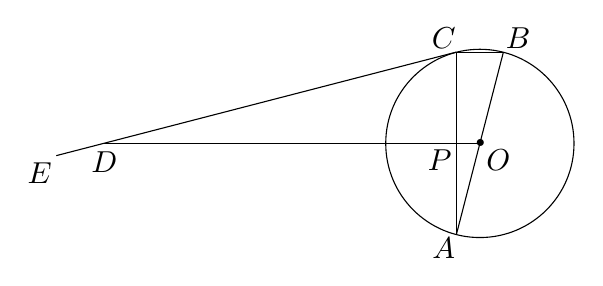
\begin{tikzpicture}[x=1pt, y=1pt,
    every node/.style={inner sep=0pt, font=\fontsize{10.5pt}{12.6pt}\selectfont}]

  % ---- 圆：m + 4c + h（源内容流 path 41，lw 0.398） ----
  % 源真页坐标：m (695.7345,608.2880)
  %   c (695.7345,627.0750) (680.5055,642.3040) (661.7185,642.3040)
  %   c (642.9305,642.3040) (627.7015,627.0750) (627.7015,608.2880)
  %   c (627.7015,589.5010) (642.9305,574.2720) (661.7185,574.2720)
  %   c (680.5055,574.2720) (695.7345,589.5010) (695.7345,608.2880)  h
  \draw[line width=0.398pt]
    (68.0330,34.0160)
    .. controls (68.0330,52.8030) and (52.8040,68.0320) .. (34.0170,68.0320)
    .. controls (15.2290,68.0320) and (0.0000,52.8030) .. (0.0000,34.0160)
    .. controls (0.0000,15.2290) and (15.2290,0.0000) .. (34.0170,0.0000)
    .. controls (52.8040,0.0000) and (68.0330,15.2290) .. (68.0330,34.0160)
    -- cycle;

  % ---- AC（源 path 42，lw 0.398）：A(653.2134,575.2900) → C(653.2134,641.2860) ----
  \draw[line width=0.398pt] (25.5119,1.0180) -- (25.5119,67.0140);

  % ---- BC（源 path 43，lw 0.398）：B(670.2226,641.2860) → C(653.2136,641.2860) ----
  \draw[line width=0.398pt] (42.5211,67.0140) -- (25.5121,67.0140);

  % ---- AB（源 path 44，lw 0.398）：A(653.2134,575.2900) → B(670.2224,641.2860) ----
  \draw[line width=0.398pt] (25.5119,1.0180) -- (42.5209,67.0140);

  % ---- DO（源 path 45，lw 0.398）：O(661.7180,608.2880) → D(525.6440,608.2880) ----
  \draw[line width=0.398pt] (34.0165,34.0160) -- (-102.0575,34.0160);

  % ---- EC 切线（源 path 46，lw 0.398）：C(653.2134,641.2860) → E(508.6344,603.8660) ----
  \draw[line width=0.398pt] (25.5119,67.0140) -- (-119.0671,29.5940);

  % ---- 标签：源文本 Tm 原点（基线左端），CMMI10 10.5pt ----
  \node[anchor=base west] at (16.6435,-7.5010)  {$A$};   % 源 (644.3450,566.7710)
  \node[anchor=base west] at (43.2065,68.3580)  {$B$};   % 源 (670.9080,642.6300)
  \node[anchor=base west] at (16.4485,68.3580)  {$C$};   % 源 (644.1500,642.6300)
  \node[anchor=base west] at (-106.5505,23.4550) {$D$};  % 源 (521.1510,597.7270)
  \node[anchor=base west] at (-129.5855,19.6660) {$E$};  % 源 (498.1160,593.9380)
  \node[anchor=base west] at (36.2065,24.0880)  {$O$};   % 源 (663.9080,598.3600)
  \node[anchor=base west] at (15.0715,24.0880)  {$P$};   % 源 (642.7730,598.3600)
  % 圆心点：源 CMSY10 0x0F（`\bullet`），Tm 为 0.6 缩放（CMSY10 10.5pt × 0.6），
  % 基线原点 (660.1428,606.8878) → 本地 (32.4413,32.6158)。
  \node[anchor=base west, scale=0.6] at (32.4413,32.6158) {$\bullet$};

\end{tikzpicture}
%
% 【自验结果】
%   探针：latexmk -pdfxe，0 error / 0 Overfull / 0 Underfull / 0 Missing character；
%         页面 200.38 × 82.72 pt（standalone border=0）。
%   tex 反算：6 条路径 + 8 个标签全部匹配，最大残差 0.000000 pt（阈值 0.05）。
%   600dpi 墨迹：整体墨迹包围盒最大边差 0.209 pt；几何包围盒 0.123 pt；
%         标签中心最大 0.295 pt（D）。（尺度归一，已扣除探针
%         0.996276 = 72/72.27 的 TeX pt / PDF bp 均匀因子）
%         按页面 bp 直接比较（物理）最大 0.679 pt，全部来自该 0.37% 均匀缩放。
%   灵敏度：端点 E +0.15pt → tex 检查器报 0.1500、600dpi 几何包围盒报 0.2409；
%         标签 C +0.15pt → tex 检查器报 0.1500、600dpi 标签中心报 0.0868。均能报出。
\end{center}
\nopagebreak[4]
\end{question}
\gkpart{三、解答题}

\begin{question}
\gkti{16}在平面直角坐标系 \(xOy\) 中，已知向量 \(\boldsymbol{m}=\left(\dfrac{\sqrt{2}}{2},-\dfrac{\sqrt{2}}{2}\right)\)，\(\boldsymbol{n}=(\sin x,\cos x)\)，\(x\in\left(0,\dfrac{\pi}{2}\right)\)。

（1） 若 \(\boldsymbol{m}\perp\boldsymbol{n}\)，求 \(\tan x\) 的值；

（2） 若 \(\boldsymbol{m}\) 与 \(\boldsymbol{n}\) 的夹角为 \(\dfrac{\pi}{3}\)，求 \(x\) 的值。

\end{question}
\begin{question}
\gkti{17}某工厂 36 名工人的年龄数据如下表。

\begin{center}
\begingroup\setlength{\tabcolsep}{4pt}
\begin{tabular}{cccccccc}
\toprule
工人编号 & 年龄 & 工人编号 & 年龄 & 工人编号 & 年龄 & 工人编号 & 年龄 \\
\midrule
1 & 40 & 10 & 36 & 19 & 27 & 28 & 34 \\
2 & 44 & 11 & 31 & 20 & 43 & 29 & 39 \\
3 & 40 & 12 & 38 & 21 & 41 & 30 & 43 \\
4 & 41 & 13 & 39 & 22 & 37 & 31 & 38 \\
5 & 33 & 14 & 43 & 23 & 34 & 32 & 42 \\
6 & 40 & 15 & 45 & 24 & 42 & 33 & 53 \\
7 & 45 & 16 & 39 & 25 & 37 & 34 & 37 \\
8 & 42 & 17 & 38 & 26 & 44 & 35 & 49 \\
9 & 43 & 18 & 36 & 27 & 42 & 36 & 39 \\
\bottomrule
\end{tabular}
\endgroup
\end{center}

（1） 用系统抽样法从 36 名工人中抽取容量为 9 的样本，且在第一分段里用随机抽样法抽到的年龄数据为 44，列出样本的年龄数据；

（2） 计算（1）中样本的均值 \(\bar{x}\) 和方差 \(s^2\)；

（3） 36 名工人中年龄在 \(\bar{x}-s\) 与 \(\bar{x}+s\) 之间有多少人？所占的百分比是多少（精确到 \(0.01\%\)）？

\Needspace{0.4\textheight}
\end{question}
\begin{question}
\gkti{18}如图，三角形 \(PDC\) 所在的平面与长方形 \(ABCD\) 所在的平面垂直，\(PD=PC=4\)，\(AB=6\)，\(BC=3\)。点 \(E\) 是 \(CD\) 边的中点，点 \(F\)，\(G\) 分别在线段 \(AB\)，\(BC\) 上，且 \(AF=2FB\)，\(CG=2GB\)。

（1） 证明：\(PE\perp FG\)；

（2） 求二面角 \(P-AD-C\) 的正切值；

（3） 求直线 \(PA\) 与直线 \(FG\) 所成角的余弦值。
\nopagebreak[4]
\begin{center}% f2015gdl_q18_solid.tex — 2015 年高考数学·广东卷·理科 第 18 题（四棱锥 P-ABCD 立体图）
%
% 【来源】`.work/phase3-b17/source/2015广东理.pdf`（SHA-256
%   1c3faab50a5d1fb2bdba424104c10910341e7362d222e018fb27e631578daa9a），
%   第 2 页（合订本页 948）第 1 栏；内容对象 21。
%
% 【坐标口径】清单坐标为「真页 pt、原点左上、y 向下」。本图取
%   X0 = 202.0221（顶点 A 的 x），Y0 = 284.7441（顶点 A 的 y_top），
%   本地坐标  (x, y) = (x_page − X0, Y0 − y_top)，即本地原点 = 顶点 A，
%   x 向右、y 向上，1 单位 = 1 TeX pt。
%   换算示例：A (202.0221,284.7441) → (0,0)；B (365.2908,284.7441) → (163.2687,0)；
%   C (389.7813,243.9270) → (187.7592,40.8171)；D (226.5127,243.9270) → (24.4906,40.8171)；
%   P (308.1470,171.9323) → (106.1249,112.8118)。
%
% 【与广东文卷 Q18 的关系】本图几何与 `2015_广东卷_文科` Q18 图相同（x 逐点相同），
%   整体在页面上比文卷版下移 10.627pt；理科版新增 E（CD 中点）、F、G 三要素与
%   P–E、G–F 两条线段。文理互证由主会话事后完成，图源照本卷源件独立实测。
%
% 【线宽/虚线】全部棱 line width = 0.3985pt；DC 短段 dash pattern =
%   on 2.98883pt off 2.98883pt，dash phase = 0pt；无填充、无 c 算子（全为 m/l 直线）。
%
% 【照源复刻的存疑项】
%   DC 自 D 起为虚线：虚线路径为「交点 → D」（源 m (240.1184,597.9630)
%   l (226.5127,597.9630) 方向照录），相位 0 起于交点。
%   源未画棱 PB，照录不补。
%   源每条棱路径起点有零长度重复 moveto，按规范不复刻。
%
% 【自验结果】见文件末尾。
%
% 元素计数：11 条路径（9 条实线棱/线段 + DC 实线 + DC 虚线）、8 个标签。
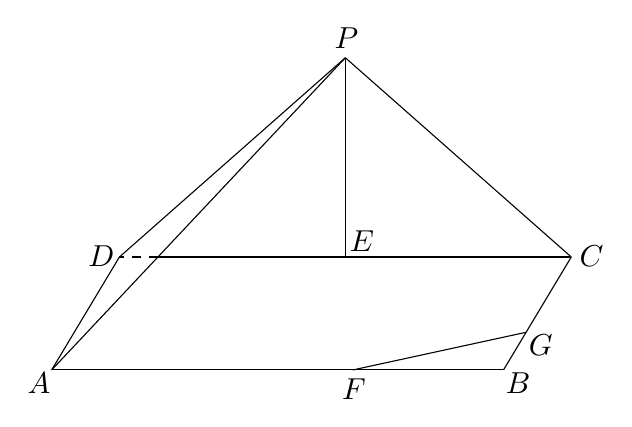
\begin{tikzpicture}[x=1pt, y=1pt,
    every node/.style={inner sep=0pt, font=\fontsize{10.5pt}{12.6pt}\selectfont}]

  % ---- 顶点（本地坐标） ----
  % A (0,0)  B (163.2687,0)  C (187.7592,40.8171)  D (24.4906,40.8171)
  % P (106.1249,112.8118)  E (106.1249,40.8171)  F (108.8458,0)  G (171.4322,13.6057)

  % ---- P–D（源 path 0：m D(226.5127,597.9630) l P(308.1470,669.9577)，本图反向） ----
  \draw[line width=0.3985pt] (106.1249,112.8118) -- (24.4906,40.8171);

  % ---- P–C（源 path 1：m P(308.1470,669.9577) l C(389.7813,597.9630)） ----
  \draw[line width=0.3985pt] (106.1249,112.8118) -- (187.7592,40.8171);

  % ---- A–D（源 path 2：m A(202.0221,557.1459) l D(226.5127,597.9630)） ----
  \draw[line width=0.3985pt] (0.0000,0.0000) -- (24.4906,40.8171);

  % ---- A–B（源 path 3：m B(365.2908,557.1459) l A(202.0221,557.1459)，本图反向） ----
  \draw[line width=0.3985pt] (0.0000,0.0000) -- (163.2687,0.0000);

  % ---- G–F（源 path 4：m G(373.4543,570.7516) l F(310.8679,557.1459)） ----
  \draw[line width=0.3985pt] (171.4322,13.6057) -- (108.8458,0.0000);

  % ---- A–P（源 path 5：m A(202.0221,557.1459) l P(308.1470,669.9577)） ----
  \draw[line width=0.3985pt] (0.0000,0.0000) -- (106.1249,112.8118);

  % ---- B–C（源 path 6：m B(365.2908,557.1459) l C(389.7813,597.9630)） ----
  \draw[line width=0.3985pt] (163.2687,0.0000) -- (187.7592,40.8171);

  % ---- P–E（源 path 7：m P(308.1470,669.9577) l E(308.1470,597.9630)） ----
  \draw[line width=0.3985pt] (106.1249,112.8118) -- (106.1249,40.8171);

  % ---- D–C 实线段（源 path 8：m C(389.7813,597.9630) l (240.1184,597.9630)） ----
  \draw[line width=0.3985pt] (187.7592,40.8171) -- (38.0963,40.8171);

  % ---- D–C 虚线段（源 path 9：m (240.1184,597.9630) l D(226.5127,597.9630)，方向照源） ----
  \draw[line width=0.3985pt, dash pattern=on 2.98883pt off 2.98883pt, dash phase=0pt]
    (38.0963,40.8171) -- (24.4906,40.8171);

  % ---- 标签：源文本 Tm 原点（基线左端），CMMI10 10.5pt ----
  \node[anchor=base west] at (102.0249,116.1981) {$P$};  % 源 (304.0470,673.3440)
  \node[anchor=base west] at (13.0239,37.2291)   {$D$};  % 源 (215.0460,594.3750)
  \node[anchor=base west] at (190.6049,37.2291)  {$C$};  % 源 (392.6270,594.3750)
  \node[anchor=base west] at (-8.8691,-8.5189)   {$A$};  % 源 (193.1530,548.6270)
  \node[anchor=base west] at (163.9539,-8.5189)  {$B$};  % 源 (365.9760,548.6270)
  \node[anchor=base west] at (107.5829,42.8651)  {$E$};  % 源 (309.6050,600.0110)
  \node[anchor=base west] at (104.7409,-10.5619) {$F$};  % 源 (306.7630,546.5840)
  \node[anchor=base west] at (172.2359,5.0871)   {$G$};  % 源 (374.2580,562.2330)

\end{tikzpicture}
%
% 【自验结果】
%   探针：latexmk -pdfxe，0 error / 0 Overfull / 0 Underfull / 0 Missing character；
%         页面 210.45 × 133.43 pt（standalone border=0）。
%   tex 反算：10 条路径 + 8 个标签全部匹配，最大残差 0.000050 pt（阈值 0.05）。
%   600dpi 墨迹：整体墨迹包围盒最大边差 0.325 pt；几何包围盒 0.065 pt；
%         标签中心最大 0.298 pt（C）。（尺度归一，已扣除 0.996277 的
%         TeX pt / PDF bp 均匀因子）
%         按页面 bp 直接比较（物理）最大 0.655 pt，来自该 0.37% 均匀缩放。
%   灵敏度：顶点 C x +0.15pt → tex 检查器报 0.1500、600dpi 几何包围盒报 0.1204；
%         标签 E y +0.15pt → tex 检查器报 0.1500、600dpi 标签中心报 0.0946；
%         G–F 线宽 +0.02pt → 等效宽度 0.9094 → 0.9517 pt（delta +0.0423）。均能报出。
\end{center}
\nopagebreak[4]
\end{question}
\begin{question}
\gkti{19}设 \(a>1\)，函数 \(f(x)=(1+x^2)\mathrm{e}^x-a\)。

（1） 求 \(f(x)\) 的单调区间；

（2） 证明：\(f(x)\) 在 \((-\infty,+\infty)\) 上仅有一个零点；

（3） 若曲线 \(y=f(x)\) 在点 \(P\) 处的切线与 \(x\) 轴平行，且在点 \(M(m,n)\) 处的切线与直线 \(OP\) 平行（\(O\) 是坐标原点），证明：\(m\leqslant\sqrt[3]{a-\dfrac{2}{\mathrm{e}}}-1\)。

\end{question}
\begin{question}
\gkti{20}已知过原点的动直线 \(l\) 与圆 \(C_1\)：\(x^2+y^2-6x+5=0\) 相交于不同的两点 \(A\)，\(B\)。

（1） 求圆 \(C_1\) 的圆心坐标；

（2） 求线段 \(AB\) 的中点 \(M\) 的轨迹 \(C\) 的方程；

（3） 是否存在实数 \(k\)，使得直线 \(L\)：\(y=k(x-4)\) 与曲线 \(C\) 只有一个交点？若存在，求出 \(k\) 的取值范围；若不存在，说明理由。

\end{question}
\begin{question}
\gkti{21}数列 \(\{a_n\}\) 满足 \(a_1+2a_2+\cdots+na_n=4-\dfrac{n+2}{2^{n-1}}\)，\(n\in\mathbf{N}^*\)。

（1） 求 \(a_3\) 的值；

（2） 求数列 \(\{a_n\}\) 的前 \(n\) 项和 \(T_n\)；

（3） 令 \(b_1=a_1\)，\(b_n=\dfrac{T_{n-1}}{n}+\left(1+\dfrac{1}{2}+\dfrac{1}{3}+\cdots+\dfrac{1}{n}\right)a_n\)（\(n\geqslant2\)），证明：数列 \(\{b_n\}\) 的前 \(n\) 项和 \(S_n\) 满足 \(S_n<2+2\ln n\)。

\end{question}